% !TeX spellcheck = en_GB
\documentclass{article}

\usepackage{graphicx}
\usepackage{amsmath}
\usepackage{amsfonts}
\usepackage{hyperref}
\usepackage{verbatim}
\usepackage{kpfonts}
\usepackage{listings}

\lstset{frame=tb,
	language=Bash,
	aboveskip=3mm,
	belowskip=3mm,
	showstringspaces=false,
	columns=flexible,
	basicstyle={\small\ttfamily},
	numbers=none,
	breaklines=true,
	breakatwhitespace=true,
	tabsize=4
}

\title{Data Mining, Homework \#1}
\author{Giacomo Lanciano (1487019) \and Fabio Rosato (1565173) \and Francisco Ferreres}
\date{November 13, 2016}

\begin{document}

\maketitle
\tableofcontents
\pagenumbering{roman}

\newpage
\pagenumbering{arabic}
% !TeX spellcheck = en_GB

\section{Problem 1}

We shuffle a standard deck of cards, obtaining a permutation that is uniform over all
52! possible permutations.
\begin{itemize}
	\item[1.] Define a proper probability space $\Omega$ for the above random process. What is the probability of each element in $\Omega$?
	\item[2.] Find the probability of the following events:
	\begin{itemize}
		\item[(a)] The first three cards include at least one ace.
		\item[(b)] The first five cards include exactly one ace.
		\item[(c)] The first three cards are a pair of the same rank (they are the same number or both are J, or both are Q, etc.)
		\item[(d)] The first five cards are all diamonds.
		\item[(e)] The first five cards form a full house (three of one rank and two of another rank).		
	\end{itemize}
	\item[3.] (Optional) Develop some small programs in Python to perform simulations to check your answers.
\end{itemize}


\subsection{Probability space definition}

Let $S = \{c, d, h, s\}$ be the set of card suites. Let $R = \{2, \ldots, 9, J, Q, K, A\}$ be the set of card ranks. Hence, $C = S \times R$ is the set of cards contained in a French deck. Let $\Omega$ be the probability space of this process. Therefore,
\begin{align*}
	\Omega &= Sym(C)\\
		&= \text{symmetric group of C}\\
		&= \text{collection of all permutations of the elements in C}
\end{align*}
By definition of symmetric group\cite{sym_group}, we have that
\begin{align*}
	|\Omega| = |C|! = (|S| \cdot |R|)! = 52!
\end{align*}
In addition, we have that $\Omega$ is an equiprobable space, since every permutation of $C$ has the same probability to be the result of a shuffle. Hence,
\begin{align*}
	\Pr(\omega) = \dfrac{1}{|\Omega|} = \dfrac{1}{52!} \qquad \forall \ \omega\in\Omega
\end{align*}


\subsection{Events probabilities}
\begin{itemize}
	\item[(a)] Let $A_{ij} \in \Omega$ be the event related to drawing exactly $i$ aces in the first $j$ cards of the deck $(j \geq i)$. Therefore,
	\begin{align}
		\Pr(A_{ij}) = \dfrac{\binom{4}{i} \cdot \binom{48}{j-i} \cdot j! \cdot (52-j)!}{52!} \label{aij}
	\end{align}
	
	since there are:
	\begin{itemize}
		\item $\binom{4}{i}$ ways to choose $i$ aces.
		\item $\binom{48}{j-i}$ ways to chose the remaining $j-i$ cards.
		\item $j!$ permutations of the first $j$ cards.
		\item $52-j!$ permutations of the remaining cards.
	\end{itemize}
	
	Let $A \in \Omega$ be the event related to drawing at least 1 ace in the first 3 cards. Therefore,
	\begin{align}
		\Pr(A) = \Pr(A_{13} \cup A_{23} \cup A_{33}) = \Pr(A_{13}) + \Pr(A_{23}) + \Pr(A_{33}) \label{disj1}
	\end{align}
	
	Note that we can write \ref{disj1} since the events $A_{13}, A_{23}$ and $A_{33}$ are disjoint each other. Using (\ref{aij}), we can easily compute the single probabilities and conclude that
	\begin{align*}
		\Pr(A) \simeq 0.217
	\end{align*}
	
	\item[(b)] Let $B \in \Omega$ be the event related to drawing exactly 1 ace in the first 5 cards. Therefore,
	\begin{align*}
		\Pr(B) = \Pr(A_{15}) \simeq= 0.299
	\end{align*}
	
	exploiting (\ref{aij}).
	
	\item[(c)] Let $C \in \Omega$ be the event related to drawing a "tris" in the first 3 cards. Therefore,
	\begin{align*}
		\Pr(C) = \dfrac{13 \cdot \binom{4}{3} \cdot 3! \cdot 49!}{52!} \simeq 0.0023
	\end{align*}
	
	since there are:
	\begin{itemize}
		\item 13 different ranks.
		\item $\binom{4}{3}$ ways to choose 3 cards among those with the same rank.
		\item $3!$ permutations of the first $3$ cards.
		\item $49!$ permutations of the remaining cards.
	\end{itemize}
	
	\item[(d)] Let $D \in \Omega$ be the event related to drawing only Diamonds in the first 5 cards. Therefore,
	\begin{align*}
		\Pr(D) = \dfrac{\binom{13}{5} \cdot 5! \cdot 47!}{52!} \simeq 0.0005
	\end{align*}
	
	since there are:
	\begin{itemize}
		\item $\binom{13}{5}$ ways to choose $5$ cards among the Diamonds.
		\item $5!$ permutations of the first $5$ cards.
		\item $47!$ permutations of the remaining cards.
	\end{itemize}
	
	\item[(e)] Let $E \in \Omega$ be the event related to drawing a "full" in the first 5 cards. Therefore,
	\begin{align*}
		\Pr(E) = \dfrac{13 \cdot 12 \cdot \binom{4}{2} \cdot \binom{4}{3} \cdot 5! \cdot 47!}{52!} \simeq 0.0014
	\end{align*}
	since there are:
	\begin{itemize}
		\item $13 \cdot 12$ different dispositions of 2 (out of 13) ranks.
		\item $\binom{4}{2}$ ways to choose $2$ cards among those with same rank.
		\item $\binom{4}{3}$ ways to choose $3$ cards among those with same rank.
		\item $5!$ permutations of the first $5$ cards.
		\item $47!$ permutations of the remaining cards.
	\end{itemize}		
\end{itemize}


\subsection{Events simulation in Python}
We developed a simple Python script that performs drawing simulations to check our previous answers. You can find the source code in \textit{deck.py} (see attachments).
We used the Python module \textit{pydealer}\cite{pydealer} to simulate the drawing of 5 cards from a deck of French cards. Basically, we repeated the process for a huge amount of times (e.g. a million of trials) and, for each one of the events, we counted how many times it happened.
In the end, for each one of the events, we computed its frequency by dividing the occurrences for the total number of trials.
In the pictures below, you can see the results in case of a million of trials. In that case, our script takes $\sim4$ minutes to terminate.

\begin{center}
	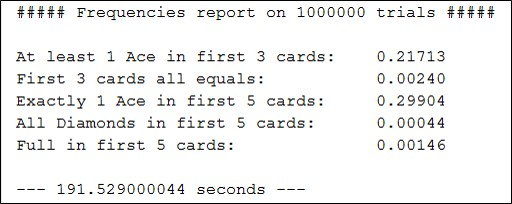
\includegraphics[]{img/deck.jpg}
\end{center}


\newpage
% !TeX spellcheck = en_GB

\section{Problem 2}

You throw a set of 3 regular dice again and again, until for the first time you see a
sum of 11 or a sum of 16.
\begin{itemize}
	\item[1.] Design an appropriate probability space for the above process.
	\item[2.] What is the probability that you stop because you see a sum of 16?
\end{itemize}

\subsection{Probability space definition}

Let $D = \{1, \ldots, 6\}$ be the set of all values that can be a result of a die throw. Let $\Omega$ be the probability space of this process. Therefore,
\begin{align*}
	\Omega = D \times D \times D
\end{align*}
since it is composed by all possible combinations of the values of 3 dice. In addition, $\Omega$ is an equiprobable space. Indeed,
\begin{align*}
	\Pr(\omega) = \dfrac{1}{|\Omega|} = \dfrac{1}{6^3} = \dfrac{1}{216} \qquad \forall \ \omega\in\Omega
\end{align*}

\subsection{Event probability}

Let $X$ be a discrete random variable representing the sum of the values of 3 dice, defined as
\begin{align*}
	X: \ \Omega \longrightarrow \{ x \in \mathbb{N} \ | \ 3 \leq x \leq 18 \}
\end{align*}
and such that
\begin{align}
	\Pr(X = x) = \dfrac{|\{ \langle y,w,z \rangle \ | \ y,w,z \in D \ \wedge \ y+w+z = x \}|}{|\Omega|} \label{triplet}
\end{align}
Let $E$, $E_i \in \Omega$ be two events such that
\begin{align*}
	E &= "stop \ because \ you \ get \ a \ sum \ of \ 16"\\
	E_i &= "you \ get \ a \ sum \ of \ 16 \ only \ at \ (i+1) \textendash th \ throw"
\end{align*}
Therefore,
\begin{align}
	\Pr(E) &= \Pr\left(\bigcup_{i = 0}^{\infty} E_i \right) \nonumber\\
		&= \sum_{i = 0}^{\infty}\Pr(E_i) \label{disj2.1}
\end{align}
Note that we can write (\ref{disj2.1}) since the events are disjoint each other.\\
Therefore, we only need to compute $\Pr(E_i)$ in order to get the desired result. Since, by definition of the problem, every throw is independent from all the others
\begin{align}
	\Pr(E_i) &= \Pr( X \ne 11 \ \cap \ X \ne 16 )^i \cdot \Pr(X = 16) \nonumber\\
			&= [1 - \Pr( X = 11 \ \cup \ X = 16)]^i \cdot \Pr(X = 16) \nonumber\\
			&= [1 - (\Pr(X = 11) + \Pr( X = 16))]^i \cdot \Pr(X = 16) \label{disj2.2}
\end{align}
Note that we can write (\ref{disj2.2}) since $X = 11$ and $X = 16$ are two disjoint events, because it is not possible to have a triplet (as we defined it in (\ref{triplet})) whose sum is both 11 and 16.\\
Therefore, we need to compute $\Pr(X = 11)$ and $\Pr( X = 16)$ in order to get $\Pr(E_i)$. We can trivially do it by enumerating all the triplets whose sum is 11 and 16, respectively, and then dividing by $|\Omega|$. Hence,

\begin{itemize}

	\item $X = 11$
	\begin{align*}
		\underbrace{
			\begin{aligned}
				\langle 1,4,6 \rangle\\
				\langle 2,3,6 \rangle\\
				\langle 2,4,5 \rangle
			\end{aligned}
		}_{ 3! \ permutations \ each}
		&&\underbrace{
			\begin{aligned}
				\langle 1,5,5 \rangle\\
				\langle 3,3,5 \rangle\\
				\langle 3,4,4 \rangle
			\end{aligned}
		}_{ 3 \ permutations \ each}\\
	\end{align*}
	\begin{align*}
		\Pr(X = 11) &= \dfrac{3 \cdot 3! + 3 \cdot 3}{216} = \dfrac{1}{8}
	\end{align*}
	
	\item $X = 16$
	\begin{align*}
		\underbrace{
			\begin{aligned}
				\langle 4,6,6 \rangle\\
				\langle 5,5,6 \rangle
			\end{aligned}
		}_{ 3 \ permutations \ each}
		&&\Pr(X = 16) = \dfrac{2 \cdot 3}{216} = \dfrac{1}{36}
	\end{align*}

\end{itemize}
Therefore, from (\ref{disj2.2}), we can conclude that
\begin{align}
	\Pr(E_i) &= \left( 1 - \dfrac{1}{8} - \dfrac{1}{36} \right)^i \cdot \dfrac{1}{36} = \left( \dfrac{61}{72} \right)^i \cdot \dfrac{1}{36} \label{pr_ei}
\end{align}
and, because of (\ref{pr_ei}), that
\begin{align}
	\Pr(E) = \dfrac{1}{36} \cdot \sum_{i = 0}^{\infty}\left( \dfrac{61}{72} \right)^i = \dfrac{1}{36} \cdot \dfrac{1}{1 - \dfrac{61}{72}} \simeq 0.18 \label{pr_e}
\end{align}
Note that we can write (\ref{pr_e}) since we obtained a convergent geometric series.\\



















\newpage
% !TeX spellcheck = en_GB

\section{Problem 3}

A group of n man and m women go to a Chinese restaurant and sit in a round table,
such that each person has to other person next to him/her.
\begin{itemize}
	\item[1.] Describe a sample space that describes the random process.
	\item[2.] Find the expected number of men who will be sitted next to at least one woman.
\end{itemize} 


\subsection{Probability space definition}

Let $S = \{1, \ldots, n+m\}$ be the set of people sitted at the table. Let $\Omega$ be the probability space of this process. Therefore,
\begin{align*}
	\Omega &= Sym(S)\\
	&= \text{symmetric group of S}\\
	&= \text{collection of all permutations of the elements in S}
\end{align*}
i.e. it consists in all possible permutations of the people sitting around the table (assuming, without loss of generality, an order among the seats).\\
By definition of symmetric group\cite{sym_group}, we have that
\begin{align*}
	|\Omega| = (n+m)!
\end{align*}
In addition, we have that $\Omega$ is an equiprobable space, since every permutation of the people has the same probability to be chosen (at random). Therefore,
\begin{align*}
	\Pr(\omega) = \dfrac{1}{|\Omega|} = \dfrac{1}{(n+m)!} \qquad \forall \ \omega\in\Omega
\end{align*}


\subsection{Expectation}

Let $X$ be a discrete random variable representing the total number of men sitted next to at least a woman, defined as
\begin{align*}
	X: \Omega \rightarrow \{ x \in \mathbb{N} \ | \ 0 \leq x \leq n \}
\end{align*}
Let $X_i$ be a Bernoulli random variable representing whether the $i\text{-} th$ man is sitted next to at least a woman or not. Hence,
\begin{align*}
	X_i = 
	\left\{ \begin{aligned}
		1 &\quad\text{if man is sitted next to at least a woman}\\
		0 &\quad\text{otherwise}
	\end{aligned}\right.
\end{align*}
Therefore, we have that
\begin{align}
	X = \sum_{i = 1}^{n}X_i \quad\Rightarrow\quad E\left[ X \right] = \sum_{i = 1}^{n} E\left[ X_i \right] \label{lin_expect}
\end{align}
Note that we can write (\ref{lin_expect}) because of the linearity of expectation.\\
Therefore, we need to compute $E\left[ X_i \right]$ in order to get the desired expected value.
\begin{align}
	E\left[ X_i \right] &= \sum_{k \in \mathrm{range}(X_i)} k \cdot \Pr(X_i = k)\nonumber\\
	&= \Pr(X_i = 1)\nonumber\\
	&= 1 - \Pr(X_i = 0)\nonumber\\
	&= 1 - \dfrac{(n+m) \cdot \binom{n-1}{2} \cdot 2 \cdot (n+m-3)!}{(n+m)!} \label{pr_xi0}\\
	&= 1 - \dfrac{(n-1) \cdot (n-2)}{(n+m-1) \cdot (n+m-2)} \label{expect_xi}
\end{align}
Let us focus on result (\ref{pr_xi0}). We trivially computed $\Pr(X_i = 0)$, i.e. the probability that a man is not seated next to a woman, by enumerating all cases in which the $i \text{-} th$ man is sitted next to other two men. Indeed, there are:
\begin{itemize}
	\item $n+m$ possible seats for the $i \text{-} th$ man.
	\item $\binom{n-1}{2}$ ways to choose other two men.
	\item 2 ways to arrange other two men ("around" the $i \text{-} th$ man).
	\item $(n+m-3)!$ permutations of the remaining people.
\end{itemize}
Hence, substituting (\ref{expect_xi}) into (\ref{lin_expect}), we have that
\begin{align*}
	E\left[ X \right] = \left( 1 - \dfrac{(n-1) \cdot (n-2)}{(n+m-1) \cdot (n+m-2)} \right) \cdot n
\end{align*}


\newpage
% !TeX spellcheck = en_GB

\section{Problem 4}

\newpage
\addcontentsline{toc}{section}{References}
\begin{thebibliography}{9}

	\bibitem{sym_group}
	\url{https://en.m.wikipedia.org/wiki/Symmetric_group}
	
	\bibitem{pydealer}
	\url{https://pypi.python.org/pypi/pydealer/}
	
	\bibitem{bbc}
	\url{http://www.bbc.co.uk/food/recipes/}
	
	\bibitem{urllib2}
	\url{https://docs.python.org/2/library/urllib2.html}
	
	\bibitem{beaut_soup}
	\url{https://pypi.python.org/pypi/beautifulsoup4}
	
	\bibitem{csv}
	\url{https://pypi.python.org/pypi/unicodecsv/0.14.1}
	
	\bibitem{nltk}
	\url{http://www.nltk.org/}
	
	\bibitem{inv_ind}
	\url{https://en.wikipedia.org/wiki/Inverted_index}
	
	\bibitem{doc_term}
	\url{https://en.wikipedia.org/wiki/Document-term_matrix}
	
	\bibitem{tf_idf}
	\url{https://en.wikipedia.org/wiki/Tf-idf}
	
	\bibitem{pickle}
	\url{https://docs.python.org/2/library/pickle.html}
	
	\bibitem{iir}
	Manning C. D., Prabhakar R., Hinrich S.,
	\emph{An Introduction to Information Retrieval},
	Cambridge University Press, Cambridge, England,
	Online edition,
	2009.

\end{thebibliography}


\end{document}
